\chapter{Void methods}
\section{Floating – point}
Pada bab terakhir kita telah membahas beberapa masalah yang berkaitan dengan angka namun tidak termasuk kedalam bilangan bulat. Kita akan membahas masalah dengan mengukur bagian yang termasuk pecahan, solusi umumnya adalah dengan menggunakan floating - point, yang dapat mewakili bilangan bulat ataupun pecahan. Dalam Java, floating – point dapat disebut juga dengan double, yang merupakan kependekan dari double - precision.

Kita dapat membuat variabel floating – point dan menetapkan nilai untuk digunakan oleh syntax yang sama dan kita gunakan pada tipe lainnya. Sebagai contoh :\newline

	double pi;
	
	pi = 3.14159:\newline \newline	
berikut ini juga merupakan pendeklarasian variabel dan menetapkan nilai pada saat bersamaan:\newline

	int x = 1;
	
	String empty = "";
	
	double pi = 3.14159;\newline \newline
Syntax ini adalah syntax yang umum; deklarasi dan penetapan biasa disebut dengan \textbf {inisialisasi}.

Meskipun floating - point (bilangan pecahan) sangat berguna, mereka juga dapat membingungkan karena terdapat pencampuran diantara bilangan bulat dan bilangan pecahan. Sebagai contoh, jika kita memiliki nilai 1, nilai tersebut termasuk kedalam sebuah integer (bilangan bulat), floating - point (bilangan pecahan), atau termasuk keduanya?

Java membedakan nilai integer (1) dengan nilai floating - point (1.0), bahkan kedua angka tersebut memiliki jumlah yang sama. Mereka termasuk kedalam jenis yang berbeda, kita tidak diperbolehkan untuk menggunakan kedua jenis bersamaan. Sebagai contoh, yang tidak diperbolehkan :\newline

	int x = 1.1;\newline \newline
karena jenis variabel yang berada pada sisi kiri adalah int (integer) dan nilai yang berada pada sisi kanan adalah double (floating – point). Tetapi mudah untuk melupakan hal ini, terutama karena Java secara otomatis dapat mengkonversi dari satu jenis ke yang lain. Sebagai contoh:\newline

	double y = 1;\newline \newline
Secara teknis hal diatas tidak legal, namun dalam Java memungkinkan dengan mengkonversi jenis variabel int (integer) ke jenis variabel double (float). Hal ini dapat memberikan kemudahan, tetapi dapat menyebabkan masalah, sebagai contoh:\newline

	double y = 1 / 3;\newline \newline
Mungkin kita berharap variable y akan bernilai 0.333333, yang merupakan suatu nilai floating-point (pecahan), tetapi kenyataannya terdapat nilai 0.0. Alasannya adalah bahwa pendeklarasian pada sisi sebelah kanan adalah rasio untuk dua bilangan bulat, jadi Java membaca sebagai divisi interger, yang menghasilkan nilai integer 0. Dikonversikan ke floating-point, hasilnya adalah 0,0.

Untuk menyelesaikan masalah ini (setelah anda memahaminya) adalah dengan membuat nilai pada sisi kanan menjadi nilai yang berjenis floating-point:\newline

	double y = 1.0 / 3.0;\newline \newline
Maka nilai y akan menghasilkan 0.333333, seperti yang diharapkan.

Operasi yang telah kita pelajari seputar penambahan, pengurangan, perkalian, dan pembagian, juga cara kerja dalam nilai floating-point, meskipun anda mungkin tertarik untuk mengetahui bahwa makanisme yang mendasari benar – benar berbeda. Bahkan, sebagian besar proses dapat menggunakan perangkat keras untuk melakukan floating-point.

\section{Converting from double to int}
Seperti yang telah disebutkan, Java mengkonversikan int (integer) ke double secara otomatis jika diperlukan, karena tidak ada data yang hilang dalam terjemahan. Disisi lain, proses dari double ke int (integer) membutuhkan pembulatan. Java tidak melakukan konversi ini secara otomatis, agar dapat lebih meyakinkan, seorang programmer, harus menyadari hilangnya bagian pecahan bilangan tersebut.

Cara termudah untuk mengkonversikan sebuah bilangan pecahan ke sebuah bilangan bulat dengan menggunakan \textbf{typecast}. Typecasting, dapat disebut demikian, karena memungkinkan Anda untuk mengambil nilai dari salah satu jenis dan yang lemparkan ke jenis lain (dalam arti molding atau reformasi).

Syntax untuk typecasting akan menempatkan tipe nama dalam sebuah kurung dan menggunakannya sebagai sebuah operator. Sebagai contoh,\newline

	double pi = 3.14159;

	int x = (int) pi;\newline\newline
Operator (int) berguna untuk mengkonversi menjadi sebuah interger, jadi x akan bernilai 3.

Typecasting mengutamakan operasi aritmatika, jadi dalam contoh tersebut, nilai Phi akan dikonversikan kedalam integer terlebih dahulu, dan hasilnya adalah 60.0, bukan 62.\newline

	double pi = 3.14159;
	
	double x = (int) pi * 20.0;\newline \newline
Mengkonversi ke sebuah integer selalu rounds down. Bahkan jika fraction adalah 0.9999999. Hal ini bersifat (precendence dan rounding) dapat membuat typecasting error-prone.

\section{Math methods}
Dalam matematika, kita mungkin telah melihat fungsi seperti sin dan log, dan kita telah mempelajari untuk mengevaluasi seperti sin($Pi/2$) dan log($1/x$). Pertama, kita evaluasi ekspresi tersebut dalam kurung, disebut dengan \textbf{argument} dari fungsinya. Lalu kita akan mengevaluasi fungsi itu sendiri, baik dengan memperhatikan dalam sebuah tabel atau dengan melakukan berbagai perhitungan.

Proses ini bisa diaplikasikan dengan berulang untuk mengevaluasi fungsi yang lebih rumit seperti log($1/ sin(Pi/2)$). Pertama kita mengevaluasi argument – argument fungsi yang lebih dalam setelah itu mengevaluasi argument tersebut, dan seterusnya.
Di Java menyediakan fungsi yang menampilkan operasi matematika yang lebih umum. Fungsi ini disebut dengan \textbf{methods}. Math method yang disebut, menggunakan sebuah syntax yang sama dengan statement yang telah kita lihat:\newline

	double root = Math.sqrt(17.0);
	
	double angle = 1.5;
	
	double height = Math.sin(angle);\newline \newline
Pada baris pertama merupakan root yang ditentukan sebagai 17. Kedua mencari  sinus yang merupakan nilai angle (sudut), yang bernilai 1.5. Java mengasumsikan nilai tersebut, kita gunakan dengan sinus dan fungsi trigonometri lainnya (cos, tan) dalam radians. Untuk mengkonversi dari derajat ke radian, kita bisa membagi dua 360 atau 2Pi. Mudahnya, Java menyediakan Math.PI :\newline

	double degrees = 90;

	double angle = degrees * 2 * Math.PI / 360.0;\newline \newline
Melihat dari PI (dalam semua huruf capital). Java tidak mengenal Pi, pi, atau pie.\newline
Motode lain yang berguna dalam matematika, nilai pecahan yang mendekati integer dan mengembalikan ke int.\newline

	int x = Math.round(Math.PI * 20.0);\newline \newline
Dalam kasus ini terjadi beberapa pilihan, sebelum metode tersebut. Hasilnya adalah 63 (yang terdekat dari 62.8319).

\section{Composition}
Sama halnya dengan fungsi matematika, method dalam Java dapat dibuat, yang artinya kita dapat menggunakan satu ekspresi dari bagian yang lainnya. Sebagai contoh, kita dapat menggunakan beberapa ekspresi sebagai argument bagi sebuah method :\newline

	double x = Math.cos(angle + Math.PI/2);\newline \newline
Statement ini mengambil nilai Math.PI, membaginya dengan 2 dan menambahkan hasilnya untuk nilai dari variabel angle. Penjumlahan yang sekarang dibahas sebagai argument terhadapat cosinus. (Pi adalah nama variabel, bukan merupakan sebuah method, jadi tidak terdapat argument, bahkan tidak ada argument kosong () ).

Kita bisa juga mengambil kesimpulan bahwa satu method dan lainnya sebagai argument untuk yang lainnya.\newline

	double x = Math.exp(Math.log(10.0));\newline \newline
Dalam Java, method log selalu berdasarkan e, jadi statement ini mencari log base e dari 10 dan menaikan e sebagai kuncinya. Hasilnya yang ditujukan untuk X; Saya harap kalian mengerti apa maksudnya.

\section{Adding new methods}
Banyak method yang dapat kita gunakan dalam Java libraries, kita dapat juga menambahkan method baru. Disini kita mendefinisikan satu method: main. Method main merupakan method yang spesial, tetapi syntax yang ada sama dengan method lainnya:\newline
\begin{lstlisting}
	public static void NAME( LIST OF PARAMETERS ) {
		STATEMENTS
	}
\end{lstlisting}
Kita dapat mengubah nama dengan apa yang kita ingin untuk nama method tersebut, terkecuali kita tidak dapat menggantinya dengan Java keyword. Umumnya, method Java memulai dengan huruf kecil dan menggunakan “camel caps,” dengan menggunakan nama yang unik, contohnya, \textbf{jammingWordsTogetherLikeThis}

Gunakan pengukur yang memberikan informasi spesifik, sehingga kita dapat menyediakannya untuk digunakan (atau dipanggil) pada method baru.
Parameter main adalah String[] args, yang artinya siapapun yang memanggil main untuk menyediakan array (kita akan mempelajari array pada Chapter 12). Setiap pasangan pertama dari method tidak mempunyai parameter, syntax akan terlihat seperti ini:\newline
\begin{lstlisting}	
	public static void newLine() {	
		System.out.println(" ");	
	}
\end{lstlisting}	
Method tersebut bernama newLine, dan kurung kosong yang berarti tidak ada parameter. Mengandung satu statement, yang menampilkan String kosong, yang di indikasikan dengan “ “. Menampilkan sebuah String dengan tidak ada huruf bukan berarti semuanya tidak berguna, tetapi println tetap terbaca untuk menampilkan garis baru, jadi dengan kata lain statement yang digunakan untuk membuat garis baru.

Pada main, kita memanggil di method baru sama dengan kita memanggil method - method Java :\newline
\begin{lstlisting}
	public static void main(String[] args) {
		System.out.println("First line.");
		newLine();
		System.out.println("Second line.");
	}
\end{lstlisting}
Output nya adalah \newline

	First line.\newline

	Second line.\newline \newline
Perhatikan spasi yang ada diantara baris. Bagaimana jika kita membutuhkan banyak spasi diantara baris? Kita dapat memanggil method yang sama berulang:\newline
\begin{lstlisting}
	public static void main(String[] args) {
		System.out.println("First line.");
		newLine();
		newLine();
		newLine();
		System.out.println("Second line.");
	}
\end{lstlisting}
Atau kita dapat menuliskan sebuah method baru, dengan nama threeLine, yang mencetak tiga baris baru:\newline
\begin{lstlisting} 
		public static void threeLine() {
			newLine(); newLine(); newLine();
	}
		public static void main(String[] args) {
				System.out.println("First line.");
			threeLine();
				System.out.println("Second line.");	
	}
\end{lstlisting}
Kita harus memperhatikan beberapa hal terhadap program diatas:\newline \newline
\textbullet	Kita dapat memanggil prosedur yang sama lebih dari sekali.\newline \newline
\textbullet	Kita dapat mempunyai method yang dapat memanggil method lain. Dalam hal ini, main memanggil threeLine dan threeLine memanggil newLine.\newline \newline
\textbullet	Dalam threeLine tertulis tiga statement pada satu baris yang sama, yang artinya secara syntax legal (ingat bahwa spasi dan baris baru biasanya tidak mengganti makna dari suatu program). Biasanya merupakan hal yang bagus untuk beberapa statement jika terdapat dalam barisnya sendiri.\newline

Kita mungkin akan bertanya – tanya mengapa terdapat beberapa kerumitan dalam membuat method – method baru.
Ada beberapa alasan; contoh berikut memeberikan dua demonstrasi.\newline \newline
1.	Membuat sebuah method baru memberikan kita sebuah kesempatan untuk memberikan nama pada sebuah kelompok statement. Method dapat menyederhanakan program dengan menyembunyikan perhitungan kompleks dibalik pernyataan tunggal, dan dengan menggunakan kata – kata Bahasa Inggris ditempat kode misterius. Yang artinya, newLine atau System.out.println(“ “)?\newline \newline
2.	Membuat sebuah method baru dapat membuat program lebih ringkas dengan mengeleminasi ulang kode. Sebagai contoh, untuk menampilkan Sembilan baris baru berurutan, kita dapat memanggil theeLine sebanyak 3 kali.\newline \newline
Dalam bagian 7.6 kita akan kembali membahas pernyataan ini dan daftar beberapa tambahan keuntungan memecah program kedalam method - method.

\section{Classes and methods}
Melihat kembali semua kode program dari bagian sebelumnya, akan menjadi class seperti ini: 
\begin{lstlisting}
	class NewLine {
		public static void newLine() {
				System.out.println("");
	}
		public static void threeLine() {
			newLine(); newLine(); newLine();
	}
		public static void main(String[] args) {
				System.out.println("First line.");
			threeLine();
				System.out.println("Second line.");
		}
	}
\end{lstlisting}
Baris pertama berisi definisi dari class baru tersebut yang disebut NewLine. Sebuah class adalah kumpulan dari beberapa method yang saling terhubung. Disini, class bernama NewLine terdapat tiga method, yaitu newLine, threeLine, dan main.

Class lain yang kita punya yaitu class Math. Yang terdapat sqrt, sin, dan lainnya. Ketika kita memanggil method Math, kita menspesifikkan nama class (Math) dan nama method. Itulah kenapa syntax dengan sedikit perbedaan dalam method Java dan method – method yang kita buat:\newline

	Math.pow(2.0, 10.0);
	
	newLine();\newline\newline
Statement pertama memanggil method pow dalam Math class (yang menimbulkan argument pertama dengan argument kedua). Statement kedua memanggil method newLine , Java mengasumsikan dalam class dengan menulis (i.e., NewLine). 
Jika kita memanggil sebuah method dari class yang salah, compiler akan menghasilkan error. Sebagai contoh, jika kita mengetik:\newline

	pow(2.0, 10.0);\newline\newline
Compiler akan merespon, “Can’t find a method named pow in class NewLine.” Jika kita melihat sebuah pesan seperti ini, kita mungkin akan bertanya – tanya  kenapa hal tersebut mencari pow dalam definisi class yang kita buat tersebut.

\section{Programs with multiple methods} 
Ketika kita melihat pada sebuah definisi class yang mengandung sebagian method, yang mengharuskan untuk membacanya dari atas ke bawah, tetapi membuat bingung, karena bukan urutan eksekusi program.

Eksekusi selalu berawal pada statement pertama dari main, terlepas darimana itu adalah dalam program (dalam contoh ini sengaja ditaruh pada bagian bawah). Statement yang tereksekusi satu per satu, dalam urutan, hingga kita menemukan method invocation. Method invocation seperti jalan memutar di aliran eksekusi. Bukan pergi ke statement selanjutnya, tetapi pergi ke baris pertama method yang dipanggil/terpanggil, mengeksekusi seluruh statement yang ada disana, kemudian kembali, dan lakukan secara berulang sampai program tersebut selesai.

Terdengar cukup mudah, namun kita harus ingat bahwa satu method dapat memanggil yang lain. Jadi, apabila kita sudah ditengah - tengah main, kita mungkin harus pergi dan mengeksekusi statement di threeLine. Tapi sementara kita mengeksekusi threeLine, kita akan mendapat tiga kali kesempatan untuk pergi (keluar statement) dan menjalankan newLine (tergantung bagaimana statement main tersebut).

Pada bagian ini, newLine memanggil println, sehingga dapat menyebabkan yang lainnya belum dijalankan. Untungnya, Java dapat menyimpan sebuah pelacakan dimana pelacakan (terakhir) itu berada, jadi ketika println telah lengkap, println yang telah lengkap mengambil kembali dimana println yang telah lengkap tadi ditinggalkan didalam newLine, lalu kembali ke threeLine, dan pada akhirnya kembali ke main sehingga program dapat dihentikan.

Secara teknis, sebuah program tidak dapat dihentikan diakhir sebuah main. Sebagai gantinya, mengambil eksekusi dimana program tersebut meninggalkan sebuah program yang dipanggil oleh main, yang berarti penerjemah Java. Penerjemahan meneliti beberapa hal seperti menghapus windows dan membersihkan keseluruhan, dan kemudian programnya terhentikan.

Apakah kesimpulannya? Ketika membaca sebuah program, jangan membaca program tersebut dari atas ke bawah. Dengan kata lain, ikuti sesuai aliran eksekusi.

\section{Parameters and arguments} 
Beberapa method yang telah kita pakai, membutuhkan argument yang nilainya kita sediakan ketika kita memanggil method tersebut. Sebagai contoh, untuk menemukan angka sinus, kita harus menyediakan angka tersebut. Sehingga sinus mengambil double yang sama seperti argumennya. Untuk mencetak sebuah String, kita harus menyediakan String tersebut, jadi sebuah println mengambil sebuah String sebagai sebuah argument. 

Beberapa method mengambil lebih dari satu argument, contohnya, pow mengambil dua double, dasar dan eksponen.

Ketika kita menggunakan method, kita menyediakan argument. Ketika kita menulis sebuah method, kita mengkhususkan sebuah list dari parameter. Sebuah parameter merupakan variabel yang menyimpan sebuah argument. Sebuah list parameter mengindikasi argument apa yang dibutuhkan;

Contohnya, printTwice mengkhusukan parameter tunggal, s, yang memiliki tipe String. Kita sebut s sebagai String, tetapi kita dapat memberikan nama variabel apapun.
\begin{lstlisting}
public static void printTwice(String s) {
	System.out.println(s);
	System.out.println(s);
}
\end{lstlisting}
Ketika kita memanggil printTwice, kita dapat membuat sebuah argument tunggal dengan tipe String.\newline

	printTwice("Don't make me say this twice!");\newline\newline
Ketika kita memanggil sebuah method, argument yang telah kita sediakan ditugaskan sebagai parameter. Dalam contoh ini, argument “don’t make me say this twice!” ditugaskan sebagai parameter s. proses ini disebut \textbf {parameter passing}  karena nilai akan diteruskan dari luar method ke dalam.

Sebuah argument dapat menjadi beberapa ekspresi, jadi jika kita memiliki variabel String, kita dapat menggunakan argument tersebut:\newline

	String argument = "Never say never.";

	printTwice(argument);\newline \newline
 Nilai yang kita sediakan sebagai argument harus memiliki tipe yang sama dengan parameter. Contohnya, jika kita membuat seperti ini:\newline
	
	printTwice(17);\newline \newline
Kita mendapatkan pesan error “cannot find symbol”, yang tidak sangat membantu. Alasannya adalah Java mencari method bernama printTwice yang dapat mengambil argument integer. Sejak disana tidak terdapat satupun yang dicari, maka tidak bisa menemukan “symbol.” 
\newline
\newline
System.out.println dapat menerima beberapa tipe argument. Tetapi terdapat pengecualian; banyak mehod yang tidak begitu akomodatif.

\section{Stack diagrams}
Parameter dan variabel lain hanya terdapat didalam method itu sendiri, dalam batas – batas utama, tidak terdapat yang berupa s. Jika kita coba untuk menggunakannya, compiler akan bermasalah. Demikian pula, apabila didalam printTwice tidak terdapat sebuah argument.

Salah satu cara untuk melacak dimana setiap variabel didefinisikan adalah dengan diagram tumpuk (\textbf {Stack diagram}). Diagram tumpuk sebelumnya dicontohkan seperti ini:
\newline
\newline
\begin{figure}[h]
\centering
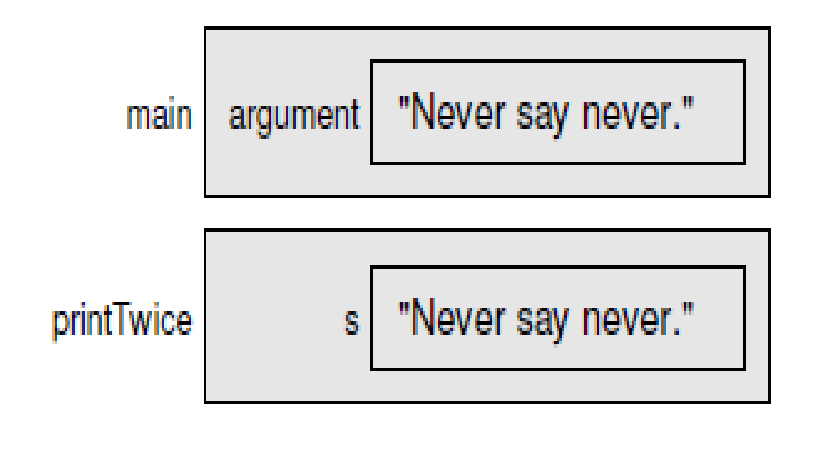
\includegraphics[width=0.4\linewidth]{stackDiagrams.png}
\label{fig:stackDiagrams.png}
\end{figure}
\newline
\newline
Masing – masing method terdapat kotak abu - abu yang disebut \textbf{frame}, yang berisikan method parameter dan variabel. Nama method berada diluar frame. Biasanya, nilai masing – masing variabel dimasukan kedalam sebuah kotak dengan nama variabel disebelahnya.

\section{Methods with multiple parameters}
Syntax yang digunakan untuk mendeklarasi dan memanggil method dengan beberapa parameter biasanya terdapat kesalahan. Pertama, ingat bahwa kita harus mendeklarasi tipe setiap parameter. Sebagai contoh:
\begin{lstlisting}
	public static void printTime(int hour, int minute) {
		System.out.print(hour);
		System.out.print(":");
		System.out.println(minute);
	} 
\end{lstlisting}
Ketika melakukan penulisan int hour, minute, tetapi formatnya hanya deklarasi variabel yang legal, bukan daftar parameter.
\newline
\newline
Umumnya sumber kebingungan adalah dari kita yang tidak dapat mendeklarasi tipe argument. Ini adalah contoh yang salah
\begin{lstlisting}
	int hour = 11;
	int minute = 59;
	printTime(int hour, int minute); // WRONG!
\end{lstlisting}
Dalam masalah ini, Java akan memberitahukan tipe hour dan minute dengan memperhatikan pendeklarasiannya. Sehingga tidak perlu memasukan tipe ketika kita melewatkan argument tersebut. Pengkoreksian syntax seperti printTime(hour, minute).

\section{Methods that return values}
 Dari beberapa method yang digunakan, seperti method Math, memiliki nilai balikan. Method lainnya, seperti println dan newLine, melakukan proses tetapi tidak memiliki nilai balikan. Timbul beberapa pertanyaan:\newline \newline
\textbullet	Apa yang terjadi jika kita memanggil sebuah method dan kita tidak melakukan apapun dengan hasilnya (i.e. kita tidak menentukan variabel atau menggunakannya sebagai bagian dari expression yang luas) ?\newline \newline
\textbullet Apa yang terjadi jika kita menampilkan method sebagai bagian dari expression, seperti System.out.println(“boo!”) + 7 ?\newline \newline
\textbullet Bisakah kita menulis method dengan nilai balikan, atau kita bergantung dengan method seperti newLine dan printTwice?\newline

Jawaban untuk ketiga pertanyaan diatas adalah “ya, kita bisa menuliskan method dengan nilai balikan,” dan kita akan melihatnya dalam beberapa bab. Kita tinggalkan dahulu untuk menjawab dua pertanyaan lainnya dengan menganalisisnya. Faktanya, kapanpun kita mendapatkan pertanyaan tentang hal yang legal dan illegal dalam Java, jalan terbaik adalah dengan cara bertanya kepada compiler (mencobanya secara langsung dengan compiler).

\section{Glossary}
\textbf{Initialization}: Sebuah statement yang dideklarasi dengan variabel baru dan menetapkan sebuah    nilai pada saat bersamaan.\newline \newline
\textbf{Floating-point}:  Sebuah tipe variabel (atau nilai) yang dapat berisi bilangan pecahan serta bilangan bulat. Tipe yang akan kita pakai untuk floating – point adalah double.\newline \newline
\textbf{Class}: Kumpulan dari method – method yang ada. Sejauh ini, yang kita gunakan adalah class Math dan class System, dan juga kita telah menggunakan penamaan class Hello dan NewLine.\newline \newline
\textbf{Method}: Urutan pernyataan yang memiliki fungsi. Method bisa / bisa tidak memiliki parameter, dan bisa / bisa tidak memiliki sebuah nilai balikan.\newline \newline
\textbf{Parameter}: Suatu informasi atau batas sebuah method yang dibutuhkan sebelum menjalankan prosesnya. Parameter sebagai variabel: mengandung nilai dan memiliki tipe.\newline \newline
\textbf{Argument}: Nilai yang telah kita sediakan ketika kita memanggil sebuah method. Nilai harus memiliki tipe yang sama sebagai parameter yang sesuai.\newline \newline
\textbf{Frame}: Struktur (yang ditunjukan dengan kotak abu – abu pada stack diagram) yang mengandung method parameter dan variabel.\newline \newline
\textbf{Invoke}: Penyebab method untuk mengeksekusi. Disini kita menggunakan istilah “memanggil”

\section{Exercises}
\textbf{Exercise 3.1.} Gambarkan frame stack yang menunjukkan state dari program dalam sub-bab 3.10 ketika main memanggil printTime dengan argument 11 dan 59.\newline \newline
\textbf{Exercise 3.2.} Point dari latihan ini adalah untuk berlatih membaca kode dan untuk meyakinkan kita mengerti alur/aliran dari proses program dengan beberapa method yang ada.\newline \newline
1.	Apa output dari program tersebut? Perhatikan tepatnya dimana ada ruang dan dimana ada baris baru.
HINT: Mulai dengan menjelaskan dalam kata – kata yang penting dan membingungkan ketika program dijalankan.\newline \newline
2.	Gambarkan diagram stack yang menunjukkan state dari program pada saat pertama kali point penting terpanggil.\newline \newline
\begin{lstlisting}
	public static void zoop() {
		baffle();
			System.out.print("You wugga ");
		baffle();
	}
\end{lstlisting}
\begin{lstlisting}
	public static void main(String[] args) {
			System.out.print("No, I ");
		zoop();
			System.out.print("I ");
		baffle();
	}
\end{lstlisting}
\begin{lstlisting}
	public static void baffle() {
		System.out.print("wug");
	ping();
	}
\end{lstlisting}
\begin{lstlisting}
	public static void ping() {
		System.out.println(".");
	}
\end{lstlisting}

\textbf{Exercise 3.3.} Point dari latihan ini adalah membuat kita mengerti bagaimana membuat dan memanggil method dengan parameter.\newline \newline
1.	Buat baris method dengan nama zool yang mempunyai tiga parameter: sebuah int dan dua yang lain (two Strings).\newline \newline
2.	Buatlah baris kode yang memanggil zool, melalui argument yang bernilai 11, nama peliharaan pertamamu, dan nama jalan tempat tinggal asalmu.\newline \newline
\textbf{Exercise 3.4.} Tujuan dari latihan ini adalah untuk mengambil kode dari latihan sebelumnya dan membuatnya dalam sebuah method yang memiliki parameter. Anda harus mengerjakan pada latihan 2.2.\newline \newline
1.	Buatlah method dengan nama printAmerican yang mencangkup day, date, month, dan year sebagai parameter dan tampilkan dalam format American.\newline \newline
2.	Cobalah method anda dengan memanggil dari main dan dengan argument yang tepat. Seharusnya output dari yang telah dibuat seperti ini (kecuali tanggal yang mungkin berbeda):\newline

Saturday, July 16, 2011 \newline \newline
3.	Saat Anda berhasil membuat printAmerican, buatlah method lain disebut printEuropean yang dapat menampilkan tanggal dalam format European.